\chapter{Computational Model based on Circuits}\label{chap:circs}
The canonical theoretical representation of a computer is the Turing
machine \cite{Turing01011937}.
Very briefly, this representation can handle general computations and is as
efficient as modern random access memory computers up to a polynomial factor.
But for a homomorphic scenario we must rely on an alternative computational
model, specially -- boolean or arithmetic -- \emph{circuits} that allows us to
represent algorithms in a algebraic form.

These primitives can also handle general computations and almost as efficiently
as Turing machines. More precisely, if there is a Turing machine program that
evaluates a function $f$ in at most $n$ steps, then there is a circuit
representing $f$ with size $\calO(n \log n)$ \cite{Pippenger:1979:RCM}. Of
course these values depend on the application we are computing. For
example, an arithmetic circuit for matrix multiplication adds essentially no
overhead, whereas a boolean circuit for integer multiplication is less
efficient than executing a single 32-bit machine assembly instruction.

In a circuit evaluation of a function or program, the number of computational
steps does not depend on the inputs of the function. Because of this one cannot
take advantage of certain optimizations used in today's computing environments.
For instance, the running time of a circuit evaluation for an ``easy'' input is
practically the same as the one with an ``hard'' input.

\section{Boolean circuits}
A \emph{boolean circuit} provides a good mathematical model of the circuitry
inside modern computers. They basically compute the boolean function of their
bit inputs using only boolean operations. Formally it can be defined as
follows.
\begin{definition}
  A boolean circuit over the set of boolean variables $X
  = \{\setSpace{x}{1}{n}\} \in \{0, 1\}^n$ is a directed acyclic graph with the
  following properties, where each node of the graph is referred to as
  a \emph{gate}.
  \begin{enumerate}[(i)]
    \item Gates with in-degree (or \emph{fan-in}) 0 are \emph{inputs}, and are
      labeled by either a variable from $X$ or by a boolean constant $c \in
      \{0, 1\}$.
    \item Gates with fan-in $k > 0$ are labeled by one of the boolean functions
      $\AND$, $\OR$, $\NOT$ on $k$ inputs. In the case of $\NOT$, $k = 1$.
    \item Gates with out-degree (or \emph{fan-out}) 0 are \emph{outputs}.
  \end{enumerate}
  The \emph{size} of a boolean circuit is the total number of gates. The
  \emph{depth} is the maximum distance from an input to an output (i.e., the
  longest directed path in the graph).

  \label{def:boolean}
\end{definition}

Usually, boolean circuits are composed of only one output gate, and in such
cases, it perfectly represents a boolean function
$\function{f}{\{0,1\}^n}{\{0,1\}}$.

\section{Arithmetic circuits}
Many computational problems can be written down naturally as multivariate
polynomials in the input variables. The \emph{arithmetic circuit} is
a mathematical model that captures a natural class of algorithms that only use
algebraic operations of the underlying field -- addition and multiplication --
to compute a function. Formally it is defined as follows.
\begin{definition}[{\autocite[Definition~1.1]{Shpilka:2010}}]
  An arithmetic circuit $f$ over the field $\bbF$ and the set of variables $X
  = \{\setSpace{x}{1}{n}\} \in \bbF^n$ is a directed acyclic graph with the following
  properties, where each node of the graph is referred to as a \emph{gate}.
  \begin{enumerate}[(i)]
    \item Gates with in-degree 0 are \emph{input gates}, and are labeled by
      either a variable from $X$ or a constant field element $c \in \bbF$.
    \item Every other gate is labeled by either $\times$ (\emph{product
      gate)} or $+$ (\emph{sum gate)}, and have in-degree $k = 2$.
    \item Gates with out-degree 0 are \emph{output gates}.
  \end{enumerate}
  An arithmetic circuit is called a \emph{formula} if it is a directed tree
  whose edges are directed from the leaves to the root.
  The \emph{size} of the circuit is the total number of gates, and the
  \emph{depth} is the maximum distance from an input gate to an output gate.
  \label{def:arith-circ}
\end{definition}

%\section{Arithmetic and boolean circuits}
%Formally an arithmetic circuit is defined as follows.
%
%\begin{definition}[{\autocite[Definition~1.1]{Shpilka:2010}}]
%  An arithmetic circuit $f$ over the field $\bbF$ and the set of variables $X
%  = \{\setSpace{x}{1}{n}\}$ is a directed acyclic graph with the following
%  properties. The nodes of the graph are called \emph{gates}. Every gate in $f$
%  of in-degree 0 is labeled by either a variable from $X$ or a field element
%  from $\bbF$.  Every other gate in $f$ is labeled by either $\times$ or $+$
%  and has in-degree 2.  An arithmetic circuit is called a \emph{formula} if it
%  is a directed tree whose edges are directed from the leaves to the root.
%  \label{def:arith-circ}
%\end{definition}
%
%Gates with in-degree 0 are called \emph{input} gates and gates with out-degree
%0 are called \emph{output} gates. Input gates labeled by variables in $X$ take
%arbitrary values in $F$ while gates labeled by a field element only take
%a fixed constant value $c \in \bbF$. Gates with in-degree and out-degree
%greater than 0 are \emph{internal} gates.  Each internal gate labeled by
%$\times$ is called a \emph{product} gate and every gate labeled by $+$ is
%called a \emph{sum} gate.
%
%The \emph{size} of the circuit is simply the total number of gates. The
%\emph{depth} of the circuit is the length of the longest path from input to
%output.
For our work, we are specially interested in circuits with just one output
gate, which represents the single output of a function that we wish to
authenticate in the setting of homomorphic authentication. Since each input
gate can only take arbitrary values in $\bbF$ or some constant $c \in \bbF$, it
is easy to see that the output of each gate has a nice mathematical
interpretation: it is simply a multivariate polynomial (evaluated at the
inputs). Arithmetic circuits provide a very compact and versatile way of
representing computations that can be expressed as multivariate polynomials.

The polynomial $f \in \bbF[\setSpace{x}{1}{n}]$ is computed by an arithmetic
circuit as follows. Input gates compute the polynomial defined by their label.
Sum gates compute the polynomial obtained by the sum of the two polynomials on
their incoming wires. Product gates compute the product of the two polynomials
on their incoming wires. The output of the circuit is the polynomial contained
on the outgoing wire of the output gate. The \emph{degree of a gate} is
defined as the total degree of the polynomial computed by that gates. The
\emph{degree of the circuit} is defined as the maximal degree of the gates in
the circuit.

\begin{center}
  \centering
  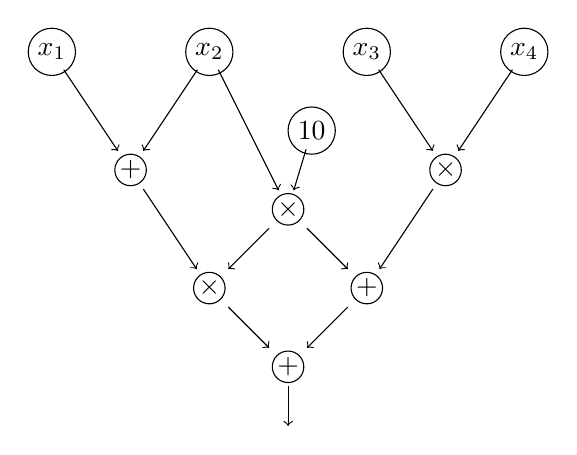
\begin{tikzpicture}
  % draw a grid starting at -4,-3 until 4,3
%  \draw[help lines] (-4,-3) grid (4, 3);

  \draw (-3, 3) circle [radius=0.3] node (x1) {$x_1$};
  \draw (-1, 3) circle [radius=0.3] node (x2) {$x_2$};
  \draw ( 1, 3) circle [radius=0.3] node (x3) {$x_3$};
  \draw ( 3, 3) circle [radius=0.3] node (x4) {$x_4$};
  \draw ( 0.3, 2) circle [radius=0.3] node (const1) {$10$};
  
  \draw ( -2, 1.5) circle [radius=0.2] node (add1) {$+$};
  \draw (  0, 1) circle [radius=0.2] node (mul1) {$\times$};
  \draw (  2, 1.5) circle [radius=0.2] node (mul2) {$\times$};

  \draw ( -1, 0) circle [radius=0.2] node (mul3) {$\times$};
  \draw (  1, 0) circle [radius=0.2] node (add2) {$+$};

  \draw (  0, -1) circle [radius=0.2] node (add3) {$+$};

  \draw[->] (x1) -- (add1);
  \draw[->] (x2) -- (add1);
  \draw[->] (x2) -- (mul1);
  \draw[->] (x3) -- (mul2);
  \draw[->] (x4) -- (mul2);
  \draw[->] (const1) -- (mul1);
  \draw[->] (add1) -- (mul3);
  \draw[->] (mul1) -- (mul3);
  \draw[->] (mul1) -- (add2);
  \draw[->] (mul2) -- (add2);
  \draw[->] (mul3) -- (add3);
  \draw[->] (add2) -- (add3);
  \draw[->] (add3) -- (0, -1.75);
\end{tikzpicture}

  \captionof{figure}[Example of an arithmetic circuit.]{
    Representation of the polynomial $f = 10x_2 (x_1 + x_2) + ((x_3 x_4)
    + 10x_2)$ as an arithmetic circuit.\label{fig:ac}
  }
\end{center}

%\section{Boolean vs Arithmetic}
Boolean circuits are not as highly structured as arithmetic circuits due to the
algebraic nature of of the latter.
That is why is is possible to prove results in the arithmetic world that are
still considered open in the Boolean world.
One very common problem related to circuits is to determine lower bounds i.e.,
prove that for a circuit computing $f$, there isn't any other better circuit.
For arithmetic circuits, there are super-linear bounds known on the size of the
circuit, while in the Boolean case, this is much harder to prove.

%\begin{definition}
%  A boolean circuit over the set of variables $X = \{\setSpace{x}{1}{n}\} \in
%  \{0, 1\}^n$ is a directed acyclic graph with the following properties.  The
%  nodes of the graph are called \emph{gates}. Every gate of in-degree (or
%  \emph{fan-in}) 0 is labeled by either a variable from $X$ or by a constant
%  $\{0, 1\}$. Gates with fan-in $k > 0$ are labeled by one of the boolean
%  functions $\AND$, $\OR$, $\NOT$ on on $k$ inputs, and in the case of $\NOT$,
%  $k = 1$. The gates with \emph{fan-out} 0 are \emph{output gates}.
%  \label{def:boolean}
%\end{definition}
%
%The notions of size and depth are exactly the same as the ones in arithmetic
%circuits.

It is worth noting that when using arithmetic circuits we are usually concerned
with polynomials of a particular form, which then fixes the set of computable
functions (i.e., polynomials in $\bbF[X]$). With Boolean circuits it is usually
the reverse, where we are interested in computing functions from $\bbF^{|X|}$
to $\bbF$.
%It is worth noting that when using boolean circuits the interest is not in any
%specific representation of the function but rather in just \emph{some}
%representation of it, while with arithmetic circuits the focus is on
%a \emph{specific} representation of the function or polynomial, i.e., we are
%concerned with polynomials a particular form, which then fixes the set of
%computable functions.
%In other words, with boolean circuits the interest is in the \emph{semantics}
%of the computation, while with arithmetic circuits the interest is on
%\emph{syntactic} computation of polynomials.
%Basically, with arithmetic circuits we usually are concerned with
%polynomials of a particular form, which then fixes the set of computable
%functions. With Boolean circuits it is usually the reverse.
%This is an important point when studying circuits because we are not interested
%in the formal computation of functions but rather in the functions that these
%circuits define.
%
In the arithmetic case, this is because a function may be expressed by
a polynomial in several ways, while, in general, a polynomial defines a unique
function. A simple example is the function $f = x^2 + x$, which defines the
zero polynomial, but only under $\bbF_2$.

%In the boolean case there is no interest in any specific polynomial
%representation of the function but rather in just \emph{some} representation of
%it, while in the arithmetic scenario the focus is on a \emph{specific}
%representation of the function. That is, with boolean circuits the interest is
%on the \emph{semantics} of the polynomial computation, while in arithmetic
%circuits the interest is on the \emph{syntactic} of the computation. This is
%important to be stressed out since we are not interested in the formal
%computation of polynomials rather than the functions that these polynomials
%define.
%It is important to stress that arithmetic circuits should be seen as computing
%\emph{specific} polynomials in $\bbF[X]$ rather than functions from
%$\bbF^{|X|}$ to $\bbF$. Essentially, one is interested in the formal
%computation of polynomials rather the functions that these polynomials define.

%When the field is $\bbF_2$ and every gate of the circuit as at most two inputs,
%the circuit is a \emph{boolean circuit}. While these circuits provide a nice
%mathematical model of a program inside a modern computer, they are not of much
%(practical) interest to us since they only handle the evaluation of binary
%functions. We will instead rely on the previously introduced arithmetic
%circuits where instead of using a binary field like in boolean circuits they
%use a field $\bbF_p$, for a given $p$\footnote{One can easily observe that an
%arithmetic circuit over $\bbF_2$ can be seen a boolean circuit}.

For arithmetic circuits, a natural question that may arise is: since there are
only $+$ and $\times$ gates, why not add a $\div$ gate to the set of allowed
operations? In the past this model was actually considered, but if we add
a $\div$ gate, this gate now computes a rational function instead of
a polynomial.  Also the problem of dividing by a zero polynomial arises, so
there needs to be a restriction for this case. But as it turns out, it is
possible to represent the division gate using only $+$ and $\times$ gates, with
some polynomially additional cost. These solutions were first introduced by
Strassen, and later by Hrube\u{s} and Yehudayof (see
\cite[Section~2.5]{Shpilka:2010} for details on both solutions and proof
sketches).

From now on we will only focus on arithmetic circuits, and so when using the
term circuit we are referring to an arithmetic circuit.

\section{Circuit Evaluation}\label{sec:circeval}
We already know how circuits are represented and what operations they compute.
But how do we efficiently evaluate them? This is critical for us because the
evaluation of a circuit shouldn't become too slow when comparing to a native
evaluation (i.e., evaluation a function on a Turing machine model). This is
even more critical as circuits start to grow, reaching sizes in the orders of
hundreds of inputs and thousands of gates.

If we look at the circuit representation, it is simply a \nom{DAG}{Directed
Acyclic Graph} that represents the dependencies between gates. That is, the
inputs of a gate $g$ are its dependencies, and therefore we cannot evaluate $g$
before we evaluate its inputs. So we can treat a circuit as a \emph{dependency
graph}. For such graphs it is possible to generate an \emph{evaluation order}
using some topological sort algorithm. Some of these algorithms perform checks
to detect whether the graph is cyclic or not, but for our case we always assume
that graphs are acyclic. These kind of algorithms are fundamental for many of
common computing applications such as program (re)compilation, system package
management or spreadsheet calculators.

The common algorithm used for topological sort is based on the
\nom{DFS}{Depth-First Search}~\cite{tarjan1972depth}, a depth search algorithm
over graphs. Basically, edges are explored out of the most recently visited
vertex $g$ that still has unexplored edges leaving it. When all of $g$'s edges
have been visited, the search ``backtracks'' to explore edges leaving the
vertex from which $g$ was explored. This process continues until all the
vertices that are reachable from the original source have been visited. If
a vertex is left unvisited, then it is used as a new source for the DFS and the
``backtracking'' process is repeated again. This process is repeated until all
vertices in the graph have been visited. The running time of DFS is $\Theta(V
+ E)$ with $V$ the number of vertices and $E$ the number of edges. A simple DFS
can be implemented as shown in \refalg{alg:dfs}.

\begin{algorithm}
  \begin{algorithmic}[1]
    \Function{DFS}{G}\Comment{Acyclic graph $G = (V,E)$}
      \For{each vertex $u \in V$}
        \State $u.color \gets$ WHITE
      \EndFor
      \State $time \gets 0$\Comment{Global variable to keep track of time}
      \For{each vertex $u \in V$}
        \If{$u.color$ == WHITE}
          \State \Call{DFS-Visit}{$G$, $u$}
        \EndIf
      \EndFor
    \EndFunction
    \Statex
    \Function{DFS-Visit}{$G,u$}
      \State $time \gets time + 1$
      \State $u.d \gets time$\Comment{Time at which white vertex $u$ was discovered}
      \State $u.color \gets$ GRAY
      \For{each vertex $v \in G.Adj[u]$}
        \If{$v.color$ == WHITE}
          \State \Call{DFS-Visit}{$G, v$}
        \EndIf
      \EndFor
      \State $u.color \gets$ BLACK\Comment{Vertex $u$ is finished}
      \State $time \gets time + 1$
      \State $u.f \gets time$\Comment{Time at which black vertex $u$ was
        finished}
    \EndFunction
  \end{algorithmic}
  \caption{Basic DFS.}
  \label{alg:dfs}
\end{algorithm}


By the end of DFS there are two timestamps in each vertex $u$: $u.d$ represents the
time at which it was first visited and $u.f$ represents the time at which all
of its children edges where visited. For each vertex $u$, it holds that
$u.d < u.f$ and their values are in $\{ 1, \dotsc, 2\abs{V} \}$.

%\begin{center}
%  \centering
%  %\input{Graphics/example-dfs}
%  \missingfigure{execute DFS on the example circuit}
%  \captionof{figure}[Depth First Search on a simple directed acyclic graph.]{
%    DFS of a DAG.\label{fig:dfs}
%  }
%\end{center}

A topological sort of a DAG $G = (V, E)$ is a linear ordering of all its
vertices such that if $G$ contains an edge $(u, v)$, then $u$ appears before
$v$ in the ordering. Any DAG has at least one topological ordering. Given an
arithmetic circuit, its topological sort can be viewed as an ordering of its
gates along a horizontal line so that all directed edges go from left to right.
%Considering the arithmetic circuit from \reffigure{fig:ac}, one of the possible
%topological orderings is:
%
%\begin{center}
%  \centering
%  %\input{Graphics/example-tsort}
%  \missingfigure{execute topo-sort on the example circuit}
%  \captionof{figure}[Topological sort of a simple directed acyclic graph.]{
%    Topological sort of a DAG.\label{fig:tsort}
%  }
%\end{center}

With DFS, a topological sorting becomes as simple as the following:
\begin{algorithm}
  \begin{algorithmic}[1]
    \Function{Topo-Sort}{$G$}
      \State \Call{DFS}{$G$}\Comment{To compute the finishing times $u.f$ for
      each vertex of $G$}
      \State Output a list $L$ in order of decreasing finishing times
    \EndFunction
  \end{algorithmic}
  \caption{A simple topological sorting algorithm, using DFS as in
    algorithm~\ref{alg:dfs}.}
  \label{alg:tsort}
\end{algorithm}


Since DFS takes time $\Theta(V + E)$ and the insertions on the list $L$ take
time $\calO(1)$, the total running time of a topological sorting based on a DFS
is $\Theta(V + E)$.

Finally, to perform the circuit evaluation we simply evaluate each gate in the
order defined by the list $L$ obtained with \textsc{Topo-Sort}. Each gate
evaluation result is kept on a list, where the last index corresponds to the
circuit's output gate.

We will be using \citetool{parno:howell:gentry:raykova:2013} to generate
circuits, and in that case, there is practically no advantage in using
a topological sorting algorithm to perform the evaluation because most of the
the circuits from \citetool{parno:howell:gentry:raykova:2013} are already
properly sorted. However, if using custom designed circuits or circuits
generated by some other means, it is necessary to generate a topological
ordering to be able to efficiently evaluate the circuit.

The reason why we are solely interested in arithmetic circuits is because they
allows to represent computations as multivariate polynomials that can be
efficiently computed. This is very important specially for our homomorphic
scenario.

\section{Circuit generation}
Even though arithmetic circuits are quite clean and simple in theory, there are
not many tools to easily compile a piece of code into a circuit representation.
At this moment, the ones from \textcite{parno:howell:gentry:raykova:2013}
(\citetool{parno:howell:gentry:raykova:2013}) and from \textcite{tinyram}
(\citetool{tinyram}) are the most efficient.

\textcite{tinyram} functionality is clearly superior because it is essentially
a port of the gcc\footnotemark compiler. Basically, \citetool{tinyram} takes
a \texttt{C} program and compiles it to a specific \citetool{tinyram} assembly
language, which is equivalent to an arithmetic circuit. Unfortunately, we
cannot easily access the arithmetic circuit but only its binary representation.
\footnotetext{\url{https://gcc.gnu.org/}}

%At this moment, the most complete and with support for more operations is the
%one of \textcite{parno:howell:gentry:raykova:2013}
%(\citetool{parno:howell:gentry:raykova:2013}).

On the other hand, \citetool{parno:howell:gentry:raykova:2013} comes equipped
with a compiler that converts a subset of the \texttt{C} language and outputs
an arithmetic circuit representation, and this is the reason why we are using
it instead of \citetool{tinyram}.
They have support for both boolean and arithmetic circuit generation, but as it
was previously mentioned, we are only interested on arithmetic circuits. They
also mention that the use of boolean circuits as opposed to arithmetic circuits
proved to be much slower, specially on their setting of verifiable computation.

The compiler, written in Python, can process a substantial subset of
\texttt{C}: global, function and block-scoped variables; arrays, struct's and
pointers; function calls, conditional loops; static initializers; arithmetic
and bit-wise operators; and pre-processor directives. The piece of code that we
wish to convert to a circuit must be inside the function \texttt{void
outsource(struct Input *, struct Output *)}. The parameters describe the input
and output values, respectively.

Because circuits only supports expressions and not mutable state and
iteration, the \texttt{C} program's semantics is restricted. There is no
support for dynamic operations (like memory allocations), and everything must
be compile-time constant (as pointers or array dereferences).

Their notion of arithmetic circuits is complemented with one more gate
operation: a \emph{split gate}. Basically, given a value $a \in \bbF_p$ where
$p$ is an integer with $k$ bits, the split gate outputs to $k$ gates, where
each of them represents the bit value $a_i$. Given such
binary values, it is possible to compute Boolean functions using only
arithmetic gates: $\mathrm{NAND}(a,b) = 1 - ab$, $\mathrm{AND}(a,b) = ab$,
$\mathrm{OR}(a,b) = 1 - (1 - a)(1 - b)$; each of these operations comes at the
cost of only one multiplication.

The recombination of the $k$ bits into a single gate is given by the expression
$\sum_{i=1}^{k}{2^{i - 1}a_i}$. As they noticed, recombining these $k$ bits
into an integer is not very costly as they only perform additions and
multiplications by constants, which are practically free.

In the setting of VC and SNARKs\footnotemark, the interest is in the
verification of computations rather than efficiently compute them
homomorphically (which is our case). That is why they introduced a split gate,
which is very efficiently verifiable and allows them to compute more
operations.  \footnotetext{\citetool{parno:howell:gentry:raykova:2013} and
\citetool{tinyram} were constructed with VC and SNARKs in mind.}

\section{Limitations}
One problem with circuit generation has to do with \emph{data dependencies}.
While the circuit's inputs do not affect its topology, they affect the program
flow and memory accesses. Thus, a circuit must be ready to support a wide range
of program flows and memory accesses, despite the fact that its topology has
already been set. The technique \citetool{parno:howell:gentry:raykova:2013}
uses to generate circuits is \emph{program analysis}.
With program analysis, if the program and its inputs are known in advance,
generating the corresponding circuit is simple: build the circuit's topology to
match the pre-determined program flow and its memory accesses. But if only the
program is known in advance, and not its inputs, the program must be analyzed
piece by piece (i.e., unroll loops, branches, etc) so that the circuit can
handle different input values. However, this technique has one big limitation.
The class of supported programs is not very broad, as
\citetool{parno:howell:gentry:raykova:2013} requires arrays accesses and loop
iterations bounds to be compile-time constants, which forces us to ``write
around'' this limited functionality.

Unfortunately, the introduction of the split gate is a limitation for us
because we are not solely interested in an efficient verification (as with VC
and SNARKs), which it limits even more the subset of \texttt{C} code that we
can convert to arithmetic circuits. This means that we cannot have conditional
dependencies which means that everything must be known at compile time (except
for the input values), and we cannot also use any bit-wise operation since they
give origin to split gates.

However, we can still write simple \texttt{C} programs and use
\citetool{parno:howell:gentry:raykova:2013} to convert them to arithmetic
circuits, so that they can be used by the \citescheme{catalano:fiore:2013}
scheme.

